\documentclass[12pt]{article}
\usepackage[utf8]{inputenc}
\usepackage{mathpazo}
\usepackage{subfig}
\usepackage[a4paper,top=3cm,bottom=3cm,left=2.5cm,right=2.5cm,marginparwidth=3cm]{geometry}
\pagestyle{myheadings}	\usepackage{tabularx}

% Paquetes
\usepackage{mathtools, amsmath, setspace, amsfonts, enumitem, listings}
\usepackage{cancel, amssymb, xfrac, enumitem, setspace, tcolorbox}
\usepackage{pdfpages, soul, graphicx, multicol, float}
\tcbuselibrary{theorems}

% Bibliography
\usepackage[spanish]{babel}
\usepackage[natbibapa]{apacite}
\bibliographystyle{apacite}

\usepackage[natbibapa]{apacite}
\bibliographystyle{apacite}

% Hipervinculos
\definecolor{udesa}{HTML}{00529B}
\usepackage[colorlinks=true, allcolors=udesa]{hyperref}
\usepackage{listings}
\usepackage[colorinlistoftodos]{todonotes}
\usepackage{parskip}

\DeclareMathOperator*{\plim}{plim}
\setlength{\parskip}{1em}

% Commands
\providecommand{\abs}[1]{\lvert#1\rvert}
\providecommand{\abs}[1]{\lvert#1\rvert}
\newcommand{\HRule}{\rule{\linewidth}{0.3mm}} 

\hypersetup{breaklinks=true,
            pdfauthor={Riquelme y Pacheco},
            pdftitle={Problem Set 5},
            colorlinks=true,
            citecolor=udesa,
            urlcolor=udesa,
            linkcolor=udesa,
            pdfborder={0 0 0}}


\markboth{4444}{Herramientas computacionales para la investigaci\'on - MAE UdeSA 2022}

\title{ %\includegraphics[scale=0.5]{Logos/Udesa_Azul.jpg}\\
%\vspace{0.5cm}
Herramientas computacionales para la investigaci\'on \\
\vspace{0.3cm}
\textbf{Tarea 1: Data visualization}}
\author{Tom\'as Pacheco y Abigail Riquelme}
\date{Fecha de entrega: 31/07/2022}

\begin{document}
\maketitle
\onehalfspace



En el paper de \citet{schwabish2014economist} se presentan tres principios básicos que se deben cumplir al realizar gráficos. El primero de ellos dice que se debe mostrar los datos de modo que el lector comprenda la historia que se está contando. Por esto, hay que mostrarlos de la forma más clara posible. Además, no es necesario mostrar todos los datos, sino aquellos que son más relevantes. 

El segundo principio dice que hay que ser ordenados. El autor recomienda evitar el uso de elementos que sean innecesarios o distractivos para el lector. El tercer principio plantea que se debe integrar el texto y el gráfico, es decir, hacer que el gráfico esté autocontenido.

Ahora bien, con el objetivo de cumplir con los tres principios anteriormente nombrados, en esta tarea, corregiremos tres gráficos realizados en clase. 

En la Figura (\ref{primerooriginal}) se presentan los siete histogramas realizados en clase. Podemos decir que no se esta cumpliendo el primer principio del \textit{paper} dado que son varios graficos para incluir en un texto, esto podria resumirse en una menor cantidad de figuras y aun asi mostrar la misma informaci\'on, con esto estar\'iamos reduciendo la carga de informaci\'on visual del lector. Teniendo en cuenta esto decidimos unificar los siete gr\'aficos en uno solo (Figura \ref{primeromod}). Adem\'as de reducir la informaci\'on visual para el lector, el tener todos los histogramas en un mismo gr\'afico permite comparar de mejor manera el monto de los pr\'estamos para diferentes grados de cr\'edito. En este caso elegimos colores con cierta transparencia para que se puedan diferenciar los siete histogramas. 

También podemos decir que el gráfico original, Figura (\ref{primerooriginal}), no cumple con el tercer principio dado que no tiene título y los nombres de los ejes no son claros, esto también fue corregido en la Figura (\ref{primeromod}). 

\begin{figure}[htbp]
    \centering
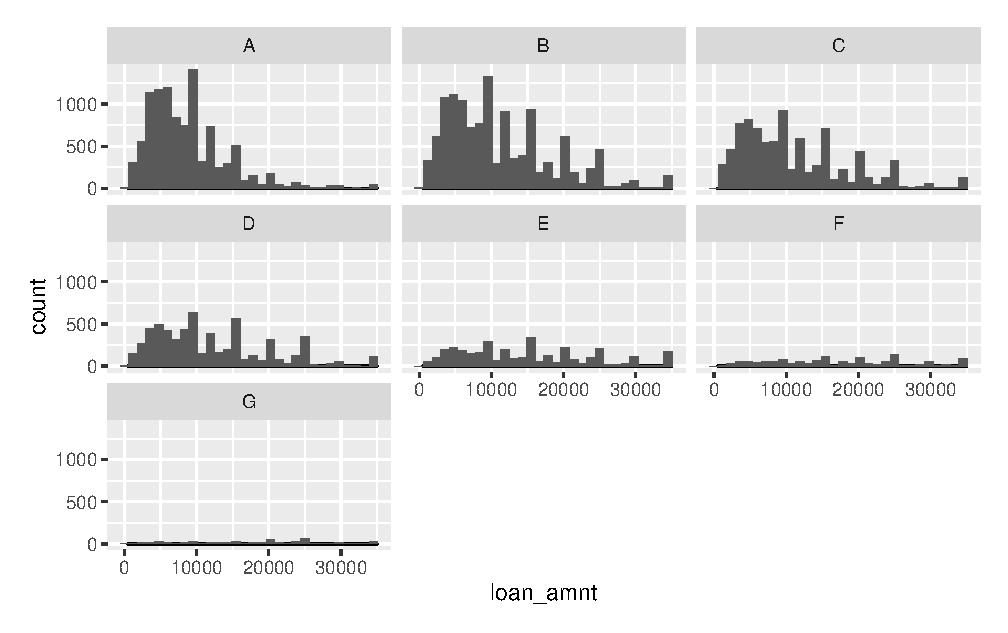
\includegraphics[width = \textwidth]{graficos/primergrafico_original.eps}
    \caption{ Primer gráfico (original)}
    \label{primerooriginal}
\end{figure}

\begin{figure}[hbtp]
    \centering
\includegraphics[width = \textwidth]{graficos/primergrafico_modificado_mod.pdf}
    \caption{ Primer gráfico (modificado)}
    \label{primeromod}
\end{figure}

En la Figura (\ref{segundooriginal}) se observa un grafico de dispersión entre el consumo de electricidad per cápita y el PBI per cápita. Se diferencia mediante colores entre cinco paises distintos. Además se presentan las lineas de tendencia para estos paises. Podemos decir que este gráfico cumple con el segundo principio dado que no se identifican elementos distractivos. Ahora bien, al igual que el gráfico anterior, no cumple con el primer ni tercer principio. Con respecto al primer principio podemos decir que la Figura (\ref{segundooriginal}) no lo cumple dado que, si suponemos que son de interes los paises China e India, no se pueden observar de manera clara estos datos. Con respecto al tercer principio, podemos decir que no lo cumple debido a que no tiene título y los títulos de los ejes no son claros. 

Teniendo en vista lo especificado en el párrafo anterior construimos la Figura (\ref{segundomod}). Para poder cumplir con el primer principio decidimos hacer un zoom para los datos con menor PBI per cápita, de esta forma se pueden observar de manera mas clara los datos de China e India. Luego, para poder cumplir con el tercer principio agregamos un título que sea informativo y corregimos los nombres de los ejes. 

\begin{figure}[htbp]
    \centering
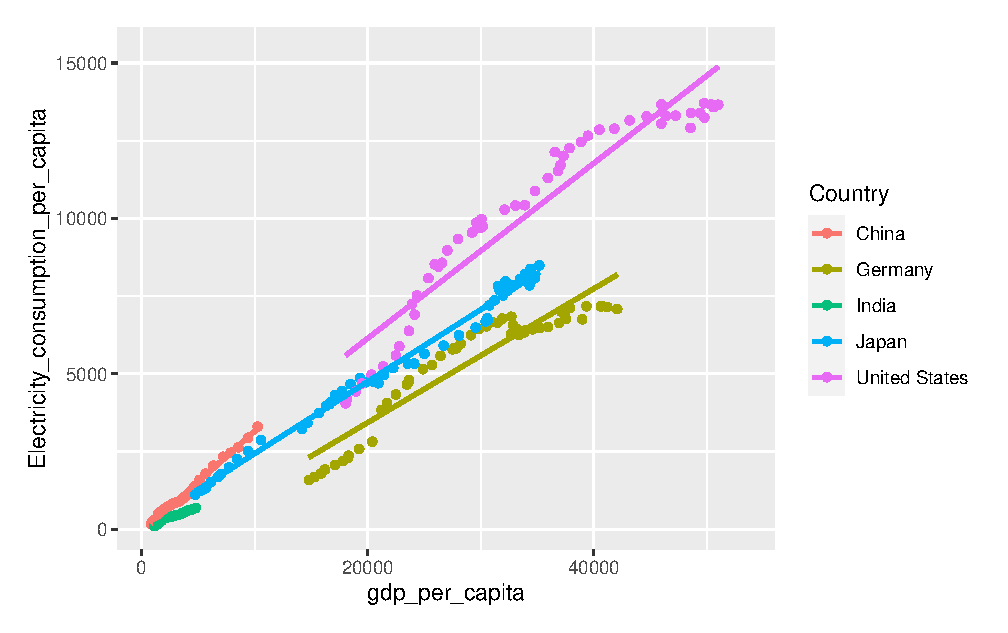
\includegraphics[width = \textwidth]{graficos/segundografico_original.eps}
    \caption{Segundo gráfico (original)}
    \label{segundooriginal}
\end{figure}

\begin{figure}[htbp]
    \centering
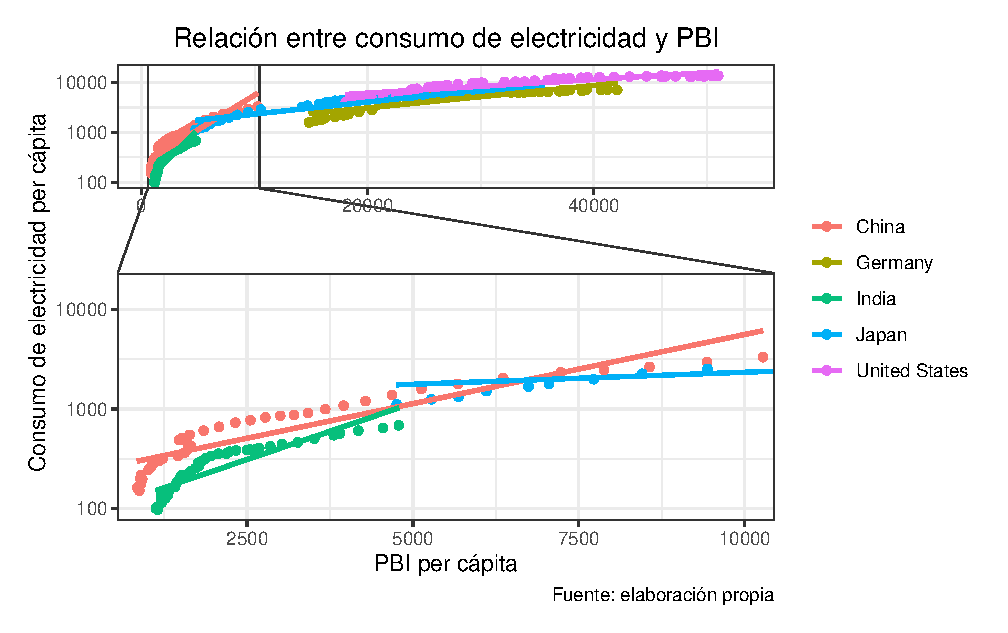
\includegraphics[width = \textwidth]{graficos/segundografico_modificado.eps}
    \caption{Segundo gráfico (modificado)}
    \label{segundomod}
\end{figure}

En la Figura (\ref{tercerooriginal}) presentamos el tercer gráfico de clase elegido para este trabajo. Este es un gráfico de dispersión entre el precio de cierre de Facebook (USD) y el mes del año. Además, se agrega el promedio en cada mes. En primer lugar, es importante notar que en ningún momento se aclara que tenemos datos de los años 2017 y 2018, es por esto que podemos decir que dicha figura no cumple con el primer principio. En cuanto al segundo y tercer principio es posible ver que se cumplen dado que no hay elementos distractivos y el gráfico está, en general, autocontenido. 

Ahora, para mejorar la claridad de la Figura (\ref{tercerooriginal}) decidimos diferenciar mediante colores aquellos datos que corresponden al año 2017 y aquellos que corresponden al año 2018. Además, incluimos el dato del promedio del precio de cierre de Facebook para cada año. 


\begin{figure}[htbp]
    \centering
\includegraphics[width = \textwidth]{graficos/tercergrafico_original_mod.pdf}
    \caption{Tercer gráfico (original)}
    \label{tercerooriginal}
\end{figure}


\begin{figure}[htbp]
    \centering
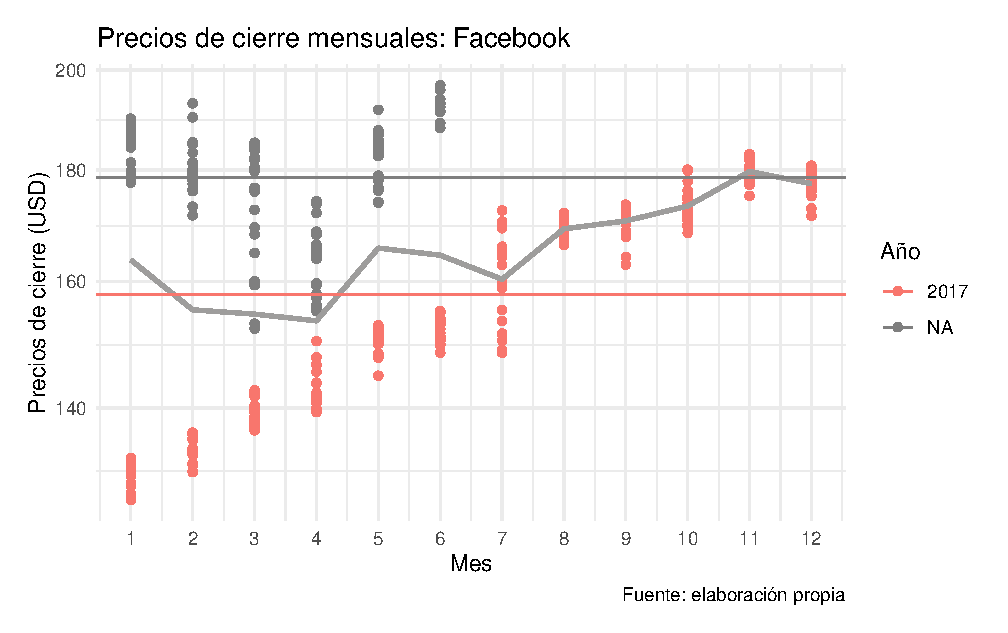
\includegraphics[width = \textwidth]{graficos/tercergrafico_modificado.eps}
    \caption{Tercer gráfico (original)}
    \label{terceromod}
\end{figure}







\bibliography{ref}
%\nocite{*}

\end{document}




